\documentclass[11pt,a4paper]{article}
\usepackage[utf8]{inputenc}
\usepackage[spanish]{babel}
\usepackage{amsmath}
\usepackage{amsfonts}
\usepackage{amssymb}
\usepackage{graphicx}
\usepackage{url}
\author{Ignacio Ramírez}
\title{Detección de Sellos}

\begin{document}
\maketitle


\section{Descripción del problema}

Los sellos de los documentos permiten saber por dónde pasó un cierto documento, es decir, nos da algo de información sobre la ruta adminstrativa de dicho documento, su función, etc.

El problema es bien simple de plantear: se trata de detectar e identificar cada uno de los sellos que se encuentra en un documento. 

La figura~\ref{fig:sellos} muestra algunos ejemplos.

\begin{figure}[ht]
\centering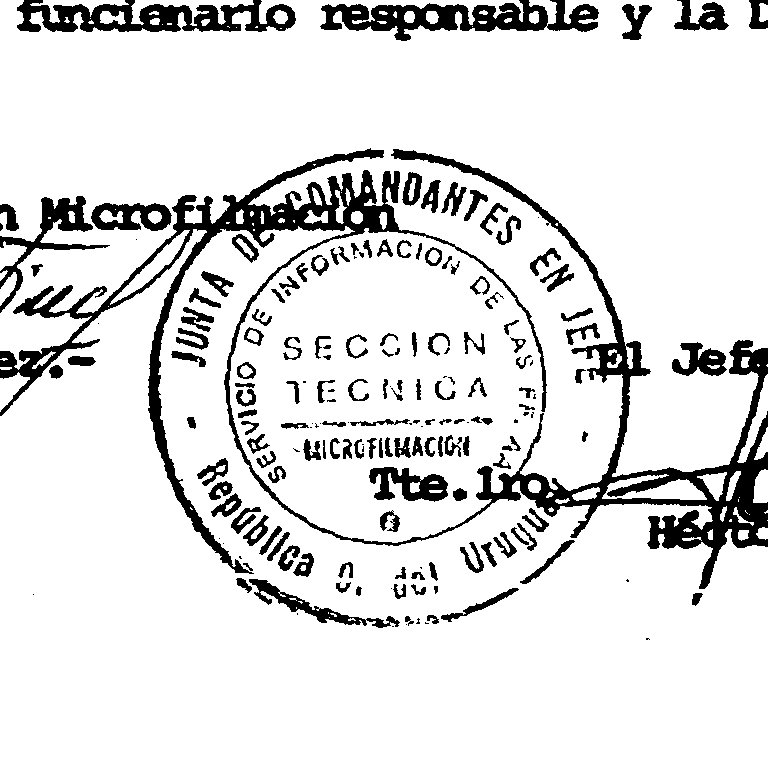
\includegraphics[width=0.3\textwidth]{sello1.jpg} %
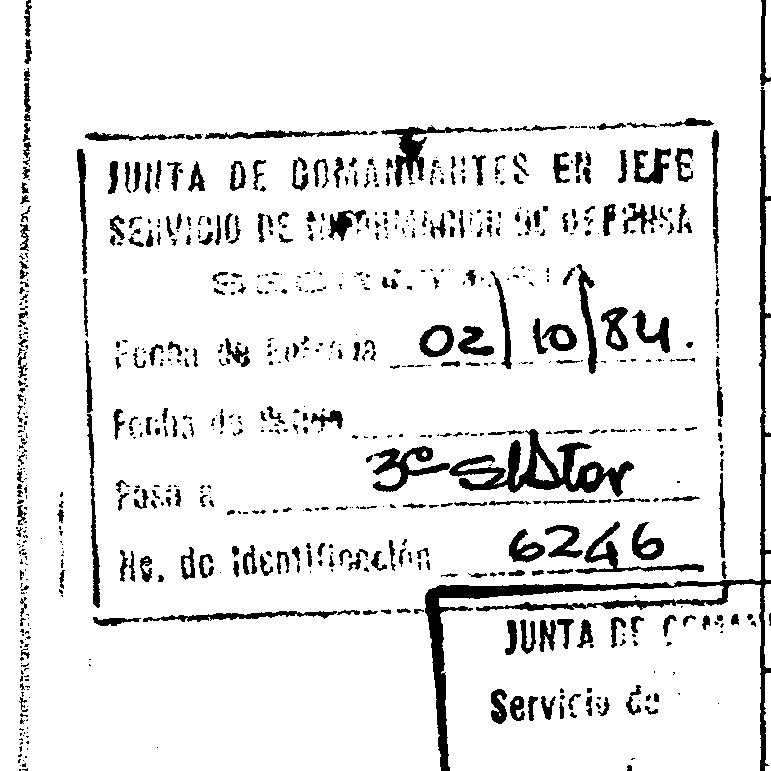
\includegraphics[width=0.3\textwidth]{sello2.jpg}\\
\centering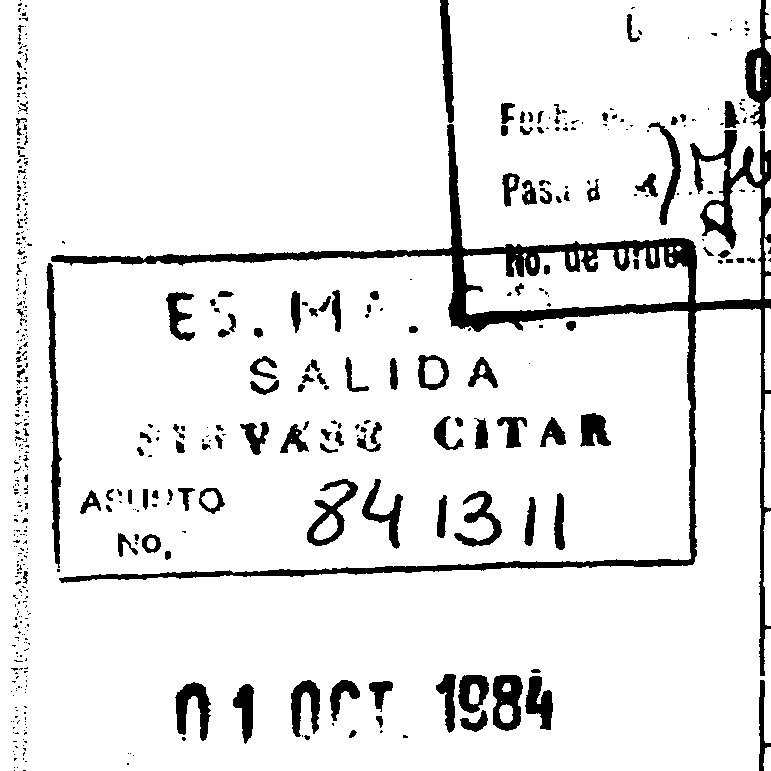
\includegraphics[width=0.3\textwidth]{sello3.jpg} %

\includegraphics[width=0.3\textwidth]{sello4.jpg}
\caption{\label{fig:sellos} Ejemplos de algunos sellos.}
\end{figure}

\section{Aspectos a considerar}

Puede resultar muy útil tener los siguientes aspectos en cuenta:
\begin{itemize}
\item La escala de todos los documentos es la misma, por lo que un mismo sello tendrá el mismo tamaño en todas las imágenes.
\item Los sellos pueden aparecer inclinados, por lo que simplemente buscar una imagen idéntica (sin tener en cuenta las posibles rotaciones) puede fallar.
\item Por otro lado, es posible que los sellos circulares puedan ser identificados sólo en base a los círculos concéntricos que suelen tener y su tamaño. Esa información, por lo menos, puede facilitar enormemente la detección (la identificación se puede hacer luego sobre un sello detectado).
\item Hay que tener en cuenta el ruido; obviamente, a nivel de pixeles, la coincidencia nunca será perfecta; hay que definir un umbral de similitud.
\end{itemize}

\section{Algunos consejos técnicos}

El método más común (y efectivo) para detectar la presencia de una cierta figura en una imagen es el denominado \emph{convolución} o \emph{filtro de apareado} (\emph{matching}). Se trata simplemente de sobreponer una copia conocida del sello buscado en \emph{todas} las posiciones posibles de la imagen y multiplicar a ambas imágenes y luego sumar los valores obtenidos de la multiplicación. En caso de coincidencia, el resultado de dicha operación será significativamente más alto que si no la hubiera.

Sobre lo anterior, dos cosas. La primera es que tal operación puede realizarse de manera muy eficiente utilizando la Transformada de Fourier. No es necesario conocer la teoría; basta con aprender a usar la función \texttt{fftconvolve} de \texttt{scipy}.\footnote{\url{https://docs.scipy.org/doc/scipy/reference/generated/scipy.signal.fftconvolve.html}}

Es muy importante tener en cuenta que los sellos pueden aparecer en varias orientaciones. En este caso no queda otra que repetir la búsqueda para distintos ángulos, rotando el sello utilizado como plantilla.

Se recomienda realizar el prototipo en Python, R, o algún otro lenguaje que ya incorpore funciones como \texttt{fftconvolve}.


\end{document}